\documentclass[a4paper,12pt,twoside,no-math]{report} 
% Specify required margin widths and setup geometry of the thesis
\usepackage{geometry}
\geometry{
	a4paper,
	left=1.25in,
	right=1in,
	top=1in,
	bottom=1in
}
\usepackage[svgnames]{xcolor}
\usepackage{graphicx, pdfpages}
% Set path/directory where all figures are stored.
\graphicspath{ {figures/} }

%%
\usepackage{titlesec}
% Format section headings with sans-serif font
\titleformat{\section}
{\Large\bfseries\sffamily}
{\thesection}{1em}{}
% Format chapter headings with sans-serif font
\titleformat{\chapter}[display]
{\Huge\bfseries\sffamily}
{\chaptertitlename\ \thechapter}{20pt}{\Huge}

% Format subsection headings with sans-serif font
\titleformat{\subsection}
{\large\bfseries\sffamily}
{\thesubsection}{1em}{}

% Format subsubsection headings with sans-serif font
\titleformat{\subsubsection}
{\bfseries\sffamily}
{\thesubsubsection}{1em}{}

\usepackage{fancyhdr}
\usepackage{float}
\usepackage{tabularx}
\usepackage{epigraph}
\setlength{\epigraphwidth}{0.6\textwidth}
\setlength{\epigraphrule}{0pt}
%%%*********************************************
\newcommand{\myopeningquote}{%
  \raisebox{-0.4\height}{\scalebox{3}{\textcolor{Silver}{``}}~~}%
}
\newcommand{\myclosingquote}{%
  \raisebox{-0.45\height}{\scalebox{3}{\textcolor{Silver}{''}}}%
}


\usepackage[framemethod=TikZ]{mdframed}

\newenvironment{Frame}[1][]{%

    \begin{mdframed}[%
        frametitle={\textsf{#1}},
        skipabove=\baselineskip plus 2pt minus 1pt,
        skipbelow=\baselineskip plus 2pt minus 1pt,
        linewidth=0.5pt,
        frametitlerule=true,
        frametitlebackgroundcolor=Silver,
        roundcorner=10pt,
        nobreak=true
    ]%
    \rmfamily
}{%
    \end{mdframed}
}
\usepackage{amsmath, amssymb, fixmath, physics, cancel}
\usepackage[no-math]{fontspec}
\usepackage{newcomputermodern}
\usepackage[scaled=1.0]{XCharter}
\usepackage[final]{microtype}
\linespread{1.3}
%$$$$$$$
\usepackage[
	pdfauthor={Aditya Dev},
	pdftitle={},
	pdfsubject={MS19022 MS Thesis},
	pdfkeywords={},
	backref=page
]{hyperref}
\renewcommand*{\backref}[1]{}
\renewcommand*{\backrefalt}[4]{{\footnotesize [%
    \ifcase #1 Not cited.%
	\or Cited on page~#2%
	\else Cited on pages #2%
	\fi%
]}}
\hypersetup{
	colorlinks = true,
	linkcolor={red!50!black},
	citecolor={blue!50!black},
	urlcolor={blue!80!black}
}
\newcommand{\refapp}[1]{Appendix~\ref{#1}}
\newcommand{\refchap}[1]{Chapter~\ref{#1}}
\newcommand{\refeq}[1]{Eqn.~\ref{#1}}
\newcommand{\reffig}[1]{Figure~\ref{#1}}
\newcommand{\refsec}[1]{Section~\ref{#1}}
\newcommand{\reftab}[1]{Table~\ref{#1}}

\renewcommand{\vec}[1]{\mathbold{#1}}
\newcommand{\mat}[1]{\mathbold{#1}}
\newcommand{\psid}{\psi ^\dagger}
\newcommand{\psibar}{\overline{\psi}}
\newcommand{\ketpsi}{\ket{\psi}}
\newcommand{\kket}[1]{\left| #1 \right\rAngle}
\newcommand{\bbra}[1]{\left\lAngle #1 \right|}
\newcommand{\ketPsi}{\kket{\Psi}}
\newcommand{\innerGlob}[2]{\left\langle #1 |  #2 \right\rAngle}
\newcommand{\oper}[1]{{\operatorname{#1}}}
\renewcommand{\H}{\oper{H}}
\newcommand{\I}{\oper{I}}
\newcommand{\Vinter}{\oper{V}}
\newcommand{\Vs}{\oper{V}_s}
\newcommand{\doubleunderbar}[1]{\underbar{\underbar{#1}}}
\begin{document}


% Use '\thispagestyle{empty}' to ensure that this page
% is not counted in page numbering.
\thispagestyle{empty}

% Set required margin widths for first few pages.
\newgeometry{top = 2.5in, left = 1.25in, right = 1in, bottom = 1in}
\begin{titlepage}

    \begin{center}
        \sffamily
        \LARGE
        \textbf{Relational Dynamics From Entangled Eigenstates}
        \vspace{1cm}
        
        \Large
        \textbf{Aditya Dev}
    
        \vspace{1cm}
        \large
        
        \textit{A dissertation submitted for the partial fulfilment of
        BS-MS dual degree in Science}
        
        \vspace{3.5cm}
    
        
\includegraphics[trim={5mm 5mm 5mm 5mm},clip,width=8cm]{HighResolutionLogo.jpg}
        \vspace{1cm}
        
        \large
        \textbf{Indian Institute of Science Education and Research, Mohali}\\
        \large
        \textbf{\today} 
    
    \end{center}
    
    
    \end{titlepage}

% Use '\thispagestyle{empty}' to ensure that this page
% is not counted in page numbering.
\thispagestyle{empty}
\cleardoublepage

% Use Roman Page Numbering for first few pages.
\pagenumbering{Roman}

{\sffamily \begin{center}
    \textbf{\Large Certificate of Examination}
\end{center}

This is to certify that the dissertation titled \textbf{Relational Quantum Dynamics From Entangled Eigenstates} submitted by 
\textbf{Aditya Dev} (Reg. No. MS19022) for the partial fulfillment of BS-MS Dual Degree 
programme of the institute, has been examined by the thesis committee duly appointed by the 
institute. The committee finds the work done by the candidate satisfactory and recommends 
that the report be accepted.

\vspace{4cm}

Dr. Abhishek Chaudhuri \hspace{0.9cm} Dr. Ambresh Shivaji \hspace{0.9cm} Dr. Ramandeep S. Johal

\vspace{4cm}

\begin{flushright}
    Dr. Abhishek Chaudhuri
    \\
    (Supervisor)
    \\
    \vspace{4cm}
    Dated: \today
\end{flushright}

\cleardoublepage

% Declaration.
\begin{center}
    \textbf{\Large Declaration}
\end{center}
The work presented in this dissertation has been carried out by me under the joint supervision of \textbf{Dr. Abhishek Chaudhuri} at the Indian Institute of Science Education and Research, Mohali, and \textbf{Prof. Dr.  Jan Micheal Rost} at Max Planck Institute for the Physics of Complex Systems, Dresden Germany. 

\vspace{0.4cm}

This work has not been submitted in part or in full for a degree, a diploma, or a fellowship to any other university or institute. Whenever contributions of others are involved, every effort is made to indicate this clearly, with due acknowledgment of collaborative research and discussions. This thesis is a bonafide record of my original work, and all sources listed within have been detailed in the bibliography.

\vspace{2cm}

\begin{flushright}
Aditya Dev
\\
(Candidate)
\\
Dated: [Enter Relevant Date]
\end{flushright}

In my capacity as the supervisor of the candidate's project work, I certify that the above statements by the candidate are true to the best of my knowledge.

\vspace{2cm}

\begin{flushright}
Dr. Abhishek Chaudhuri
\\
(Supervisor)
\\
Dated: [Enter Relevant Date]
\end{flushright}

\cleardoublepage

% Acknowledgements.
\include{acknowledgement}}
% Abstract.
%\fontfamily{ptm}\selectfont % Times font
\addcontentsline{toc}{chapter}{\textbf{Abstract}}
\begin{center}
    \textbf{\Large Abstract}
\end{center}

Use this section to include an abstract of the thesis.

\newpage
\restoregeometry

% Creates a List of All Figures.
\addcontentsline{toc}{chapter}{\textbf{List of Figures}}
\listoffigures

\newpage

% Creates a List of All Tables.
\addcontentsline{toc}{chapter}{\textbf{List of Tables}}
\listoftables

% Creates a Table of Contents.
\tableofcontents

\newpage
% Certificate of Examination.


% Use Arabic Page Numbering for the rest of the thesis.
\pagenumbering{arabic} 
% Chapter 1 - Introduction.


%%%
% This code snippet takes care of the required  
% Equation/Figure numbering scheme.
\renewcommand\thefigure{\thechapter.\arabic{figure}}    
\renewcommand{\theequation}{\thechapter.\arabic{equation}}
\setcounter{equation}{0}
\setcounter{figure}{0}
%%%
\chapter{Introduction}\label{chap:chapter1}

\epigraph{\myopeningquote Our greatest glory is not in never falling, but in rising every time we fall.\myclosingquote}
{Confucius}%



Unification of Quantum Mechanics and General Relativity has been the Holy Grail of physics for since their inception. But no satisfactory theory has ever been proposed that solves this problem? General relativity states that a physical theory should not depend on background structures. However, standard quantization techniques often rely on background structures, such as imposing the canonical commutation relations. The Hamiltonian of a generally covariant theory, such as general relativity, is constrained to vanish in the absence of boundaries. If one tries to incorporate the theory of general relativity and quantum mechanics i.e in Canonical Quantization of gravity one ends up with a Hamiltonian constraint (i.e. \(\Hat{\operatorname{\mathbf{H}}}\left|\Psi\right\rAngle = 0\)). This leads to an infamous problem known as ``the problem of time” in the canonical approach to quantum gravity. The issue is that quantum states of spacetime (and matter in it) do not seem to undergo any time evolution as dictated by the constraints of the theory.
\section{Example Section}\label{sec:example_section}
Include equations if required:
%%%
% Example Equation.

\begin{equation}
\label{eq:straight_line}
i\hbar \frac{\partial \Psi}{\partial t} = -\frac{\hbar^2}{2m} \nabla^2 \Psi + \hat{V}\Psi
\end{equation}
\[
\nabla \times \mat{B} = \mu_0 \mat{J} + \mu_0 \varepsilon_0 \frac{\partial \mat{E}}{\partial t}
\]

%%%

The issue is that quantum states~\cite{article_name} of spacetime (and matter in it) do not seem to undergo any time evolution as dictated by the constraints of the theory.
\begin{Frame}[Frame Title]
However, upon closer inspection, it is clear that the quantum theory is not 'timeless' as often stated. The problem of time is rather a manifestation of background independence and means that physical states do not evolve relative to an external background time. Instead, one must extract a time evolution in a relational manner, i.e. pick some quantised degrees of freedom to serve as an internal time.
    \begin{equation}
\label{eq:glob_ham}
    H = \sum_{k = 0}^{N-1} H_k 	\equiv \sum_{k = 0}^{N-1} \hbar 
\omega_k \sigma_{z}^{(k)}
\end{equation} 
\end{Frame}
 The use of relational time in Quantum Mechanics is a framework in which one promotes all variables to Quantum operators and later chooses one of the variables to operate like a "clock". There are various approaches to the time problem; my work focuses on the "Page-Wootters Formalism" which defines relational dynamics in terms of conditional probabilities for the clock and evolving degrees of freedom.




Include figures if required:
%%%
% Example Figure.
\begin{figure}[ht!]
    \centering
    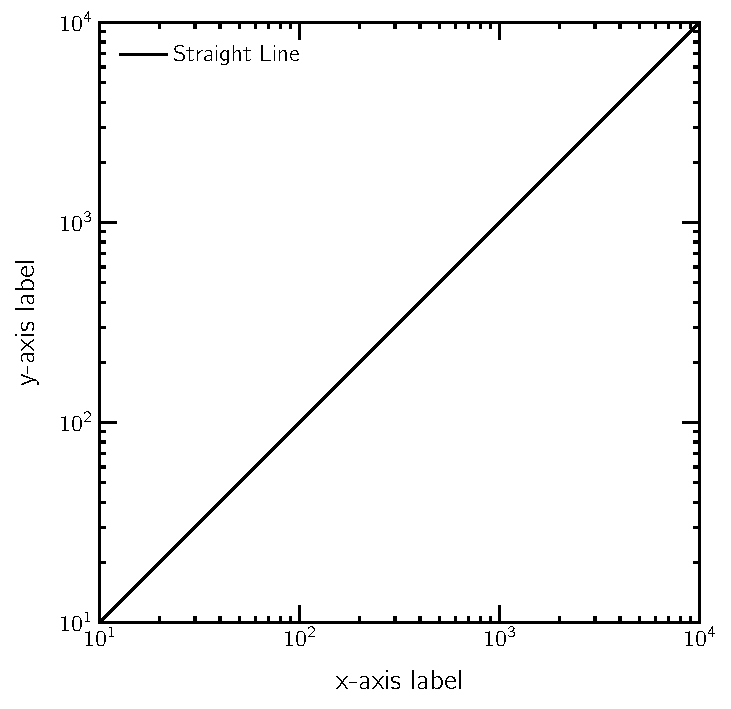
\includegraphics[width=8cm]{Chapter1/figure1.pdf}
    \caption{Example Figure: Include a caption.}
    \label{fig:example_figure}
\end{figure}
%%%

\newpage

Include tables if required:
%%%
% Example Table.
\begin{table}[ht!]
\centering
    \begin{tabular}{||c c c c||} 
     \hline
     Col1 & Col2 & Col2 & Col3 \\ [0.5ex] 
     \hline\hline
     1 & 2 & 3 & 4 \\ 
     \hline
     5 & 6 & 7 & 8 \\ 
     \hline
    \end{tabular}
\caption{Example Table: Include a caption.}
\label{table:example_table}
\end{table}
%%%

To refer to Equations/Figures/Tables, use the \verb!\ref{}! command: Equation~\ref{eq:straight_line} / Figure~\ref{fig:example_figure} / Table~\ref{table:example_table}. \verb!\ref{}! can also be used to refer to Sections: Section~\ref{sec:example_section}, Section~\ref{ssec:example_subsection}.

To cite references, use the \verb!\cite{}! command: \cite{article_name}. All cited references will automatically appear in the Bibliography section.

\subsection{Example Sub-Section}\label{ssec:example_subsection}

Create a sub-section if required.

\subsubsection{Example Sub-Sub-Section}\label{sssec:example_subsubsection}

Create a sub-sub-section if required.

\clearpage

\newpage


\renewcommand\thefigure{\thechapter.\arabic{figure}}    
\renewcommand{\theequation}{\thechapter.\arabic{equation}}
\setcounter{equation}{0}
\setcounter{figure}{0}
%%%
\chapter{Name of Chapter 2}\label{chap:chapter2}

%%%

Include as many chapters as required by using the \verb!\chapter{}! command.


\clearpage

\newpage
\chapter{Summary}\label{chap:summary}

%%%
% This code snippet takes care of the required  
% Equation/Figure numbering scheme.
\renewcommand\thefigure{\thechapter.\arabic{figure}}    
\renewcommand{\theequation}{\thechapter.\arabic{equation}}
\setcounter{equation}{0}
\setcounter{figure}{0}
%%%

Use this section to include a summary of the thesis~\cite{article_name}.


\newpage
\appendix


\chapter{Name of the Appendix Chapter}\label{app:appendix1}

%%%
% This code snippet takes care of the required  
% Equation/Figure numbering scheme.
\renewcommand\thefigure{\thechapter.\arabic{figure}}    
\renewcommand{\theequation}{\thechapter.\arabic{equation}}
\setcounter{equation}{0}
\setcounter{figure}{0}
%%%

If required, include an appendix section.


\clearpage

\newpage

\addcontentsline{toc}{chapter}{Bibliography}
\bibliographystyle{styles/bibsty.bst}
\bibliography{refrences}



\end{document}












